\chapter{Various experiments}

\section{Comparison of schedules of updates}
In the chapter $2$ different schedules of updates were analysed on toy models where the parameters of the model were known \emph{a priori} and no substantial discrepancies between asynchronous and parallel schedules were observed in terms of the quality of approximation. Taking into consideration the performance of the sequential updates on both toy models, this schedule wasn't considered in the evaluation on the real data set.

In the case of the MNIST data set, estimated magnetizations allow us to perform learning of unknown parameters. Thus, in this case we combine uncertainty related with both magnetizations and parameters -- this may lead to substantial differences in performance. Figure \ref{fig:updatesLL} shows the normalized estimates of log-likelihood of three models trained using the extended mean field approximation up to the first-order term (MF), up to the second-order term (TAP2) and up to the third-order term (TAP3), each trained with two schedules of updates.

\begin{figure}[!htb]
\minipage{0.50\linewidth}%
\includegraphics[width=\linewidth]{../../../Code/DRBM/scripts/updatesMFLL.pdf}
\endminipage 
\minipage{0.50\linewidth}  
 \includegraphics[width=\linewidth]{../../../Code/DRBM/scripts/updatesMFEMF.pdf}
\endminipage\hfill

\minipage{0.50\linewidth}%
 \includegraphics[width=\linewidth]{../../../Code/DRBM/scripts/updatesTAP2LL.pdf}
\endminipage 
\minipage{0.50\linewidth}  
\includegraphics[width=\linewidth]{../../../Code/DRBM/scripts/updatesTAP2EMF.pdf}
\endminipage\hfill

\minipage{0.50\linewidth}%
\includegraphics[width=\linewidth]{../../../Code/DRBM/scripts/updatesTAP3LL.pdf}
\endminipage 
\minipage{0.50\linewidth}  
\includegraphics[width=\linewidth]{../../../Code/DRBM/scripts/updatesTAP3EMF.pdf}
\endminipage\hfill
  \caption[Estimates of log-likelihood with different updates]{Per-sample pseudo log-likelihood (left) and EMF log-likelihood (right) on the validation set of the MNIST data divided by number of all units in the model ($1284$) across first $50$ training epochs for RBMs models trained with different schedules and number of updates. Error bars show standard deviation of $10$ trained models using a particular version of training.}
  \label{fig:updatesLL}
\end{figure}

Surprisingly, only with the naive mean field approximation we can observe that the parallel schedule provides slightly better results in terms of the approximated log-likelihood. In general, there are no significant differences between two considered schedules even though the parallel form of updates doesn't reflect the way both layers of the RBM 'communicate' with each other. Moreover, it seems that small number of fixed point iterations doesn't deteriorate the performance. This suggests that asynchronous updates with only $3$ iterative updates of magnetizations yield consistently competitive results at the same time being the most computationally inexpensive form of schedule.

\subsection{Evaluation of EMF approximation}
The similarity of the estimates of the log-likelihood using the pseudo log-likelihood method and with the extended mean field approach suggests that the high-temperature expansion might be a computationally inexpensive estimation of the partition function of the RBM and the log-likelihood in general. However, the pseudo log-likelihood is a very noisy approximation thus as a benchmark for comparison of the effectiveness of the EMF-based estimates I will use the annealed importance sampling (AIS) \cite{neal2001annealed} -- very popular method for computing the partition function. Naturally, this comparison assumes that the AIS estimate is close to the true value which in general might no be the case.
\section{Annealed importance sampling}
The AIS method is based on a very simple identity -- assume we have two distributions $p_A= \frac{1}{Z_A}p_A^*(\mathbf{x})$ and $p_B= \frac{1}{Z_B}p_B^*(\mathbf{x})$, where $p^*(\dot)$ denotes an unnormalized distribution and $Z_A, Z_B$ are partition functions of distribution $p_A$ and $p_B$ respectively. If the proposal distribution $p_A$ supports tractable sampling and tractable evaluation of both the unnormalized distribution $p_A^*(\mathbf{x})$ and the partition function $Z_A$, we can use the following relation:
\begin{align}
\begin{split}
Z_B & = \int p^*_B(\mathbf{x}) \text{d} \mathbf{x} \\ 
 &= \int \frac{p_A(\mathbf{x})}{p_A(\mathbf{x})} p^*_B(\mathbf{x}) \text{d} \mathbf{x}\\
 &=  Z_A \int \frac{ p^*_B(\mathbf{x}) }{ p^*_A(\mathbf{x}) }p_A(\mathbf{x})  \text{d} \mathbf{x} .
\end{split}
\end{align}
By sampling from the tractable distribution we can derive Monte Carlo estimator of the ratio between partition functions:
\begin{align}
\begin{split}
\frac{Z_B}{Z_A} \approx \frac{1}{N} \sum_{i=1}^N \frac{ p^*_B(\mathbf{x}^{(i)}) }{ p^*_A(\mathbf{x}^{(i)}) } = \hat{r}_{SIS},
\label{eq:ratioSIS}
\end{split}
\end{align}
where $\mathbf{x}^{(i)}$ comes from $p_A$.
Assuming that distribution $p_A$ is close to $p_B$, the estimator from  \ref{eq:ratioSIS} called simple importance sampling proves to work well \cite{minka2005divergence}. However, in high-dimensional spaces where $p_B$ is usually multimodal as it is considered in this thesis the variance of the estimator from \ref{eq:ratioSIS} might be very high. 

The idea presented above might be improved by following the classic approach from the probabilistic optimization i.e. simulated annealing. The idea is to introduce intermediate distributions that will allow to bridge the gap between two considered distributions $p_A$ and $p_B$ \cite{jarzynski1997nonequilibrium}, \cite{neal2001annealed}.

Consider a sequence of distributions $p_0, p_1, ..., p_M$ where $p_0 = p_A$ and $p_M = p_B$. If the intermediate distributions $p_{m}$ and $p_{m+1}$ are close enough, a simple estimator from \ref{eq:ratioSIS} can be used to estimate each ratio $\frac{Z_{m+1}}{Z_m}$. Using the identity: 
\begin{align}
\begin{split}
\frac{Z_M}{Z_0} = \frac{Z_1}{Z_0}\frac{Z_2}{Z_1}... \frac{Z_M}{Z_{M-1}}
\end{split}
\end{align}
those intermediate ratios are then combined to obtain the estimate of $\frac{Z_B}{Z_A}$. There is no need to compute the normalizing constants of any intermediate distributions. 
%The intermediate distributions are chosen to suit a given problem domain. 
However, in most cases we are able to draw exact samples only from the first tractable distribution $p_A$. In order to obtain samples from intermediate distributions we have to be able to generate $\mathbf{x}^{'}$ given $\mathbf{x}$ using Markov chain transition operator $T_m(\mathbf{x}^{'} |\mathbf{x}) $ that leaves $p_m(\mathbf{x})$ invariant, i.e.:
 \begin{align}
\begin{split}
\int T_m(\mathbf{x}^{'} |\mathbf{x}) p_m(\mathbf{x})\text{d}\mathbf{x} = p_m(\mathbf{x}^{'}).
\end{split}
\end{align}
These transition operators represent the probability density of transitioning from state $\mathbf{x}$ to $\mathbf{x}^{'}$ \cite{salakhutdinov2008learning}. Having obtained the sequence of samples from intermediate distributions we can obtain the improved estimator of the ratio between partition functions following the procedure:
\begin{algorithm}[!bthp]
\caption{Annealed importance sampling.}
\label{alg:vae}
\begin{algorithmic}
\State {Set $p_A$ and $p_B$ with appropriate parameters}
\For{$i \in \{1,..., N\} $} 
\State {sample $\mathbf{x}_{1}$ from $p_0 = p_A$} 
\State {sample $\mathbf{x}_{2}$ via $T_1(\mathbf{x}_{2} | \mathbf{x}_{1})$ }
\State ...
\State {sample $\mathbf{x}_{M}$ via $T_M(\mathbf{x}_{M} | \mathbf{x}_{M-1})$}
\State $r^{(i)}_{AIS} = \frac{ p^*_1(\mathbf{x}_1) }{ p^*_0(\mathbf{x}_1) }\frac{ p^*_2(\mathbf{x}_2) }{ p^*_1(\mathbf{x}_2) } ... \frac{ p^*_M(\mathbf{x}_M) }{ p^*_{M-1}
(\mathbf{x}_M) }$
\EndFor
  \State {$\hat{r}_{AIS} = \frac{1}{N} \sum_{i=1}^N \hat{r}^{(i)}_{AIS}$}
\end{algorithmic}
\end{algorithm}

It was proven that the variance of $\hat{r}_{AIS}$ will be proportional to $1 / MN$ assuming we used sufficiently large numbers of intermediate distributions $M$ \cite{neal2001annealed}. Moreover, the estimate of $Z_M / Z_0$ will be unbiased if each ratio is estimated using $N=1$ and sample $\mathbf{x}^{m}$ is obtained using Markov chain starting at previous sample. This follows from the observation that the AIS procedure is a simple importance sampling defined on an extended state space $X = (\mathbf{x}_1, \mathbf{x}_2, ..., \mathbf{x}_M)$.

The procedure described above can be adapted to the RBM case -- assume that we have estimated parameters of the model that we want to evaluate,  $\mathbf{\theta}_B$. Following \cite{salakhutdinov2008quantitative} as a tractable starting distribution $p_A$ we can use "clamped" restricted Boltzmann machine where there is no hidden layer. The sequence of intermediate distribution is then defined as:
 \begin{align}
\begin{split}
p_m(\mathbf{v}) = \frac{1}{Z_m}p^*_m(\mathbf{v}) = \frac{1}{Z_m}\sum_\mathbf{h} \exp(-E_m(\mathbf{v, h})),
\end{split}
\end{align}
where $m = 0, ..., M$, $\mathbf{h} = \mathbf{h_B}$, and the energy function has the form:
 \begin{align}
\begin{split}
E_m(\mathbf{v,h}) = (1- \beta_m) E(\mathbf{v} ;\theta_A) + \beta_m E(\mathbf{v, h} ;\theta_B),
\end{split}
\end{align}
where $\beta_m \in [0, 1]$ with $\beta_m = 0$ yielding $p_A$ and $\beta_m = 1$ giving $p_B$. By annealing slowly the "temperature" from infinity to zero, we gradually move from the state space of proposal distribution to the space defined by the untractable distribution.
% Following the approach from \ref{eq:TODOderivepropertiesofRBM} we can obtain transition operators for hidden and visible variables:
% \begin{align}
%\begin{split}
%p(h^A | \mathbf{v}) & = \sigma ((1 - \beta) NONE \\
%p(h^B) & =
%\end{split}
%\end{align}

\subsection{Comparison of AIS and EMF}
Two models were estimated based on the extended mean field approximation -- up to the second-order term (TAP2), and up to the third-order term (TAP3), to compare the quality of the approximation of the variational free energy.
Each model was re-estimated $10$ times using persistent chains with $10$ iterations of self-consistency relations with asynchronous updates. 
A sequence of $\beta$s is required to set the "tempo" of annealing -- following \cite{salakhutdinov2008learning} $1000$ $\beta_k$ were spaced uniformly from  $0 $ to  $0.5$, $4,000$ $\beta_k$ were spaced uniformly from $0.5$ to $0.9$, and $5,000$ $\beta_k$ were spaced uniformly from $0.9$ to $1.0$, with a total of 10,000 intermediate distributions. 

Firstly, both methods were compared on a small toy model -- an RBM with $15$ hidden units where we can compute the true partition function explicitly. 
Taking into consideration the inherent variability of the AIS method, $10$ runs of AIS were performed to obtain an average estimate. Figure \ref{fig:AISTAP2small} presents the true value of the partition function along with its estimates from the TAP2 and TAP3 models and using the AIS method.

\begin{figure}[!htb]
\minipage{0.50\linewidth}%
 \includegraphics[width=\linewidth]{../../../Code/DRBM/scripts/smallAISTAP2}
\endminipage 
\minipage{0.50\linewidth}  
\includegraphics[width=\linewidth]{../../../Code/DRBM/scripts/smallAISTAP3}
\endminipage\hfill
  \caption[Comparison of AIS and EMF on toy RBM]{Free energy estimates using two forms of the extended mean field approximations and AIS estimates for $10$ toy RBM models.}
  \label{fig:AISTAP2small}
\end{figure}
The results indicate that the AIS works rather well as an approximator of the true free energy. However, the EMF approximation tends to be biased and the addition of the third-order term improves the estimates only slightly. In both cases the EMF approximation consistently overestimates the true value of $\mathcal{F}$ on average by about $5\%$. 

Having justified the usage of the AIS estimate as a benchmark, we can compare both methods on the RBM with $500$ hidden units. As a sanity check, the AIS was re-estimated in this case $100$ times as the results from \cite{salakhutdinov2008learning} show that the variance is then lower than $1\%$. Figure \ref{fig:AISTAP2} presents the estimates of \ref{eq:freeEnergy} for the TAP2 and TAP3 models along with AIS estimates.

\begin{figure}[!htb]
\minipage{0.50\linewidth}%
 \includegraphics[width=\linewidth]{../../../Code/DRBM/scripts/AISTAP2}
\endminipage 
\minipage{0.50\linewidth}  
 \includegraphics[width=\linewidth]{../../../Code/DRBM/scripts/AISTAP3}
\endminipage\hfill
  \caption[Comparison of AIS and EMF on RBM with $500$ hidden units]{Free energy estimates using two forms of extended mean field approximations and AIS estimates for $10$ RBM models with $500$ hidden units.}
  \label{fig:AISTAP2}
\end{figure}

Firstly, as it was expected the learned models using two high-energy expansion yield very similar estimates of the free energy. Secondly, in both cases they give consistently biased upper bound approximation for the $\mathcal{F}$, assuming that the AIS method gives an accurate estimation of \ref{eq:freeEnergy}. As in the case of the toy model, the difference is about $5 \%$ in value on average. 
%The mean squared error between the average AIS estimate and the TAP2 method was $505.747$ while for the the approximation including third-order the MSE was $534.193$. 
This suggests that even though the extended mean field approximation enable us to learn good generative models, the approximation of the free energy is very biased. However, the computational cost of estimation is about $10^{-5}$ smaller comparing to the AIS and this method might be used if we need a ballpark figure of the value of the partition function.

\section{Deep structures}
\subsection{Unsupervised pre-training of deep neural networks}
Recent major advances in tasks like speech recognition, vision recognition or machine translation were obtained thanks to effective training of deep neural structures. Deep learning methods allow to learn high-level features based on the composition of lower level characteristics. However, the objective function in general is highly non-convex and multi-modal over high-dimensional parameter space. This naturally leads to many challenges in training such deep structures.
 
The breakthrough that lead to effective training strategies for deep architectures came in 2006 with the CD algorithm for training deep belief networks (DBN) \cite{hinton2006reducing}. The deep structure might be formed by stacking single RBMs pre-trained using contrastive divergence approach. It was empirically shown that unsupervised pre-training guides the learning towards basins of attraction of minima that support better generalization from the training data set \cite{erhan2010does}. Thus, such pre-trained networks much better generalize and are more robust comparing to networks trained only in supervised fashion.

In the previous chapter it was shown that unsupervised learning using the extended mean-field approach can be used to learn a good quality generative model of the observed phenomenon. Those results motivate learning deep structures using greedy layer-wise pre-training where instead of using CD for training RBMs we might consider fully deterministic approach. 

\subsection{Deep belief nets}
DBNs are generative graphical models with many hidden layers of hidden
causal variables which joint distribution has the following form:
\begin{align}
\begin{split}
p(\mathbf{x}, \mathbf{h}^1, \mathbf{h}^2,..., \mathbf{h}^l) = p(\mathbf{x}| \mathbf{h}^1)P(\mathbf{h}^1|\mathbf{h}^2)...
P(\mathbf{h}^{l-2}|\mathbf{h}^{l-1})P(\mathbf{h}^{l-1}|\mathbf{h}^{l}).
\end{split}
\end{align}
It was shown that adding extra layers always improve a lower bound on the log-likelihood on the training data if the number of feature detectors per layer is sufficiently large and the weights are initialized correctly.  The guarantee that we improve the bound is no longer valid if the size of subsequent hidden layers is not large enough however it was empirically proven that such approach still can learn an effective generative model. Figure \ref{fig:DBN} depicts an illustrative deep belief network. 

 \def\layersep{2.5cm}
\begin{figure}[!h]
\begin{center}
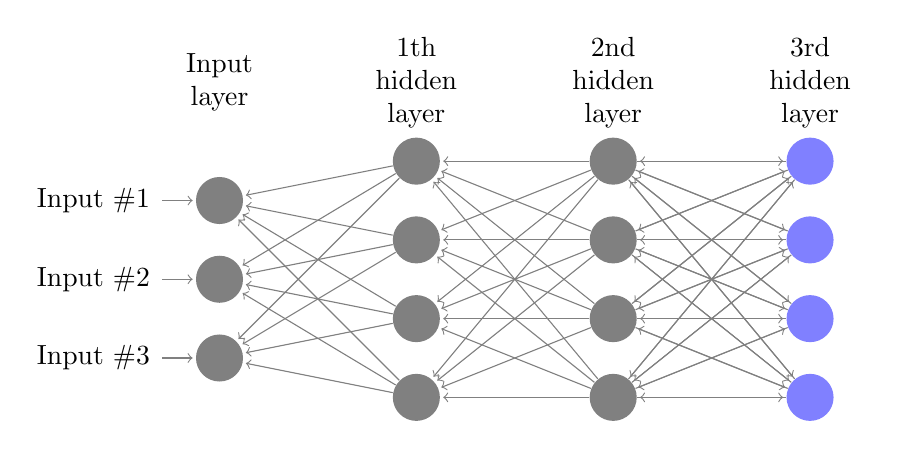
\begin{tikzpicture}[shorten >=1pt,->,draw=black!50, node distance=\layersep]
    \tikzstyle{every pin edge}=[<-,shorten <=1pt]
    \tikzstyle{neuron}=[circle,fill=blue!50,minimum size=17pt,inner sep=0pt]
    \tikzstyle{input neuron}=[neuron, fill=black!50];
    \tikzstyle{output neuron}=[neuron, fill=red!50];
    \tikzstyle{hidden neuron}=[neuron, fill=black!50];
     \tikzstyle{shidden neuron}=[neuron, fill=black!50];
          \tikzstyle{thidden neuron}=[neuron, fill=blue!50];
    \tikzstyle{annot} = [text width=4em, text centered]

    % Draw the input layer nodes
    \foreach \name / \y in {1,...,3}
    % This is the same as writing \foreach \name / \y in {1/1,2/2,3/3,4/4}       
     \node[input neuron, pin=left:Input \#\y] (I-\name) at (0,-\y) {};

    % Draw the hidden layer nodes
    \foreach \name / \y in {1,...,4}
        \path[yshift=0.5cm]
            node[hidden neuron] (H-\name) at (\layersep,-\y cm) {};

    % Draw the SECOND hidden layer nodes
    \foreach \name / \y in {1,...,4}
        \path[yshift=0.5cm]
            node[shidden neuron] (S-\name) at (2*\layersep,-\y cm) {};
            
            
    % Draw the THIRD hidden layer nodes
    \foreach \name / \y in {1,...,4}
        \path[yshift=0.5cm]
            node[thidden neuron] (T-\name) at (3*\layersep,-\y cm) {};

%    % Draw the output layer node
%    \node[output neuron,pin={[pin edge={->}]right:Output}, right of=S-3] (O) {};

    % Connect every node in the input layer with every node in the
    % hidden layer.
    \foreach \dest in {1,...,4}
    \foreach \source in {1,...,3}
            \path (H-\dest) edge  (I-\source);
            
% Connect every node in the hidden layer with every node in the
    % SECOND hidden layer.
            \foreach \dest in {1,...,4}
    \foreach \source in {1,...,4}
            \path (S-\dest) edge (H-\source) ;

% Connect every node in the hidden layer with every node in the
    % SECOND hidden layer.
    \foreach \source in {1,...,4}
        \foreach \dest in {1,...,4}
            \path (S-\source) edge (T-\dest);
      
      \foreach \dest in {1,...,4}
          \foreach \source in {1,...,4}
            \path (T-\dest) edge (S-\source) ;

    % Annotate the layers
    \node[annot,above of=H-1, node distance=1cm] (hl) {1th hidden layer};
    \node[annot,left of=hl] {Input layer};
        \node[annot,above of=S-1, node distance=1cm] (hl) {2nd hidden layer};
    \node[annot,above of=T-1, node distance=1cm] (hl) {3rd hidden layer};
\end{tikzpicture}
  \caption[Deep belief net]{An illustrative deep belief net with $3$ hidden layers where the last two layers form a single RBM.}
    \label{fig:DBN}
\end{center}
\end{figure}

Similarly to the case of the single RBM, DBN may be seen as a general approximator of any probability distribution on $\{0,1 \}^n$ and we can prove \cite{montufar2010refinements}
:
\begin{theorem} [Guido-Ay, 2010] Let $n = \frac{2^b}{2} + b$, $b \in \mathbb{N}$, $b \geqslant 1$. A DBN containing $\frac{2^n}{2(n-b)}$ hidden layers of size $n$ is a universal approximator of distributions on $\{0,1 \}^n$.
\end{theorem}

DBNs can be formed using a greedy layer-wise unsupervised training of stacked RBMs -- Algorithm \ref{alg:DBN} presents how the process folows.
\begin{algorithm}[!bthp]
\caption{Learning procedure for deep belief nets.}
\label{alg:DBN}
\begin{algorithmic}
\State {Train the first layer as an RBM, learning $P(\mathbf{x = h^{0}, h^1})$}
\For{$l \in \{2,..., L\} $} 
\State {Pass the mean activities $\mathbf{x}^l = P(\mathbf{h^{l}| \mathbf{h^{l-1}} })$ which become a representation of the input at the layer $l$.}
\State {Train the $l$-th layer treating it as an RBM with $\mathbf{x}^l$ as an input. }
\EndFor
\end{algorithmic}
\end{algorithm}
This simple and intuitive algorithm proved to be an effective way of pre-training deep structures that laid the foundations for the resurgence of deep neural networks. Originally, the building blocks are trained following contrastive divergence 
procedure.  However, the positive results obtained using the extended mean-field approximation suggests that we may follow Algorithm \ref{alg:DBN} with fully deterministic approach.

\subsection{Reconstruction analysis}
After pre-training multiple layers of feature detectors, the model can be ''unfolded'' to form an autoencoder structure where the decoder network uses transposed weights of the encoder network. At this stage, such network might be considered as feed-forward deep neural architecture and can be used as a starting point for supervised fine-tuning with respect to any training criterion that depends on the learned representation \cite{bengio2007greedy}.

To motivate the analysis of deep structures formed of stacked RBMs, I trained different three models that compress the information in the data to $25$ dimensional manifold -- using principal component analysis with first $25$ components with the highest variance, a single RBM with $25$ hidden units and a deep belief net that consists of three hidden layers of sizes $500$, $250$ and $25$. Last two models were trained using an extended mean field approach up to the second-order term with persistent magnetizations.

\begin{figure}[!htb]
\includegraphics[width=\linewidth]{../../../Code/DRBM/drbm/reconstructions2}
  \caption[Reconstructions of digits with basic models]{Reconstructions of MNIST digits (top row) generated by PCA-25 (second row),  single RBM with $25$ hiddent units (third row) and deep belief net (bottom row).}
  \label{fig:pca}
\end{figure}
As we can see, the linear transformation to the small dimensional space creates very noisy encoding system. The reconstructions show that the numbers lie very closely on the space from which we decode. The reconstructions provided by the single RBM substantially improves the quality of the reconstructions and it can be infer that the learned manifold better differentiate between the digits. However, although the background is properly delimited from the numbers, digits are still very blurry. It might be argued that the deep structure creates the most sharply-outlined numbers. From this we might infer that deep belief net is able to create more coarser and coarser features that in the process of the encoding are able to generate clear-cut digits as the learned manifold in the smallest layer is properly partitioned.

Similarly to the case of the shallow structures, we might compare the effectiveness of the EMF approach to the CD learning in the case of the greedily layer-wise training of DBN. Figure \ref{fig:drbm} presents the reconstructions of randomly chosen samples from the validation data set produced by deep autoencoders trained with four different methods for pre-training DBNs. The autoencoder consists of three hidden layers of sizes $500$, $250$ and $25$ accordingly. The extended mean field approximation was considered up to the first-order (MF), up to the second-order (TAP2) and up to the third-order (TAP3) term. One model was also trained using the CD procedure. At each layer $50$ updates through the entire data set were performed using $10$ iterations of asynchronous updates. In each case magnetization or Gibbs chains were persistent.

\begin{figure}[!htb]
\includegraphics[width=\linewidth]{../../../Code/DRBM/drbm/reconstructions}
  \caption[Reconstructions of digits with deep structures]{Reconstructions of original MNIST digits (top row) generated by four different deep belief nets trained using naive mean field approach (second row), EMF up to the second-order term (third row), EMF up to the third-order term (fourth row) and with PCD (bottom row).}
\label{fig:drbm}
\end{figure}
  
%Figure \ref{fig:drbm} presents the reconstructions of MNIST digits as well as a the original numbers. 
By the visual inspection, it might be argued that the reconstruction created by TAP2, TAP3 and PCD are of similar quality and they are more identifiable than those produced by the MF. 
It can be observed how the autoencoders learned by the EMF or the PCD recovers a a smoothed version of the original digit -- an "average" representative of a given number. Surprisingly, the addition of the third-order term leads somewhat to deterioration of the quality in reconstructions which can be observed especially in the case of the first ($2$) and sixth ($5$) number. 
The average squared errors on training and validation data sets (Figure \ref{fig:mse}) confirms the visual assessment of reconstructions. The mean field approximation obtains the highest score while TAP2 and TAP3's scores are slightly higher than with training DBN using PCD approach. 

\begin{figure}[!htb]
\begin{center}
\includegraphics[width=.5\linewidth]{../../../Code/DRBM/drbm/mseRecon}
\end{center}
  \caption[MSE of digits' reconstructions with different deep models]{MSE of reconstructions for four different models on training and validation sets.}
\label{fig:mse}
\end{figure}

Those results confirms the observations from the previous chapter and shows that additional higher-order approximations substantially improves the quality of learned magnetizations which in turns helps learning a better generative model.

ARGUMENTATION HERE FOR RICH.
%\subsection{Semi RBM}
%SEE IF IT IS WORTH IT.
%\subsubsection{Exploiting the SRBM structure}
%Clamped free energy can be written in the form:
%\begin{align}
%\begin{split}
%\mathcal{F}^c(\mathbf{v}) = & \sum_\mathbf{h} e^{-E(\mathbf{v}, \mathbf{h})} = e^{\mathbf{b}'\mathbf{v}}\sum_{h_1}...\sum_{h_m}e^{-E(\mathbf{v}, \mathbf{h})} \\
%=&  e^{\mathbf{b}'\mathbf{v}} \sum_{h_1} e^{h_1 (c_1 + W_{1\bullet}\mathbf{v})}... \sum_{h_m} e^{h_m (c_m + W_{m\bullet}\mathbf{v})} \\
%= & e^{\mathbf{b}'\mathbf{v}} \prod_{j=1}^{m} \left( 1 + e^{c_i + W_{i\bullet}\mathbf{v}} \right)
%\label{eq:freeEnergy}
%\end{split}
%\end{align}
